\section{Methodology}
Two cameras were deployed in a room of acquariums at "Fiskeri- og Søfartsmuseet" in Esbjerg to take images for building a specialized dataset and to evaluate the effects of developing a highly specialized detector rather than using a general.

\subsection{Dataset Construction}
\subsubsection{Camera}
Hardware camera can be tweaked by screwing the lens with a mechanical tool to modify it's aperture, which influences it's depth focus. 
Aperture mechanical setting (camera focus adjustment), depth control. Default not found... images well sharp enough... 50cm to infinity...

\subsubsection{Technical Challenges and their Solutions}
\textbf{Pi out of memory on image capture}
Context: tweaking camera settings, leading to larger size images
Error: mal port enable failed to enable connected port... Out of resources.
Solution: allocating more memory to the GPU by going through raspi-config Performance Options -> GPU Memory

\textbf{AWB Gains not setting}
Context: setting picamera.awg gains has no effect
Error: no change 
Solution: set awb gains after awb mode has been set to off, and capture an image. The control seems to not set before after capturing an image. Thus, setting these values and then checking the values, it might seem the modification has not been made altough it will show on the images.

\subsubsection{Image Capture}
The dataset was built by capturing images while no visitors were present in the acquarium. Due to the constraint to only operate within opening hours when the facility was open to everyone, a way to cancel image capturing was needed in the case if someone entered the room. One of the goals of the dataset was to have the images taken from the same angle as the device will be used in the future. The device was therefore mounted in the corner of the room, and ssh was used to access the device remotely from a pc in the acquarium. Then, a script was ran to capture images in sequence, storing them on the SD card in the device. The choice to store the image locally rather than transmitting it was to not have to worry about data transmission costs and issues. 

All picamera configurations used in the image capture iterations can be seen in figure TODO. Example images to display the image qualities and differences are found in appendix \ref{app:images}

\textbf{1st iteration}
\textit{Total number of images: 1312 (day 1), 986 (day 2) and 641 (day 3), total 2939. 1 subject.}

The first iteration of image capture was made with non-optimized camera configurations. To sufficiently brighten the images, the picamera.brightness attribute was set to 65. This is a postprocessing operation, which gave brighter but also artificially lit images. Also, the camera would sometimes focus on the bright fish-tanks in the museus, rendering the rest of the image rather dark. This was an effect of the awb mode and exposure mode being set to auto, and led to images of varying brightness and color. These images were still included in the dataset however, as images seen as suboptimal to the human eye may still be useful to the training of detectors. These images may be used to inspect the impact of captured image quality on inference performance. 

The images were then used to build a proof of concept for the project pipeline, verifying and developing the steps needed for a successful project. The following steps in the project pipeline are described after the description of the 2nd and 3rd iterations of image captures. 

Due to many technical difficulties the first few times images were being captured for the dataset, only the developer and author of this thesis is present in the images\footnote{Initially, an attempt was made to pass MQTT messages as a way to initialize image capture so multiple cameras could be deployed in several locations, thus speeding up and simplifying the image capturing process. This was discarded due to technical difficulties related to efficiently stopping the image capturing. For this single-deployment angle and area project, however, the approach with ssh-ing into the device worked fine.}. 


\textbf{2nd iteration}
\textit{Total number of images: 295 (normal camera) and 60 (no infrared filter camera), total 355. 4 subjects.}

For the second image-shooting session, the camera configurations had been more thorougly tested to obtain more consistent images in terms of colors and brightness. This means using non-auto auto white balancing and exposure settings, and reducing the amount of post-processing brightness adjustment. Also, some friends were invited in this session. Due to a reduced post-processing brightness augmentation, the exposure speed had to be increased to get sufficient light in the images. This meant more unclear outlines of moving subjects in the frame. It also meant more time was spent capturing and storing each image. This increased from 1.3$\frac{s}{image}$ to 6.3$\frac{s}{image}$, which means the time available for image capturing was spent less productively than with the previous camera configuration. Depending on the impacts of image consistency on inference accuracy vs. amount of training data, capturing with a higher exposure speed and then post-processing the images to be brighter might be the better solution. Also, as pointed out by TODO insert mikkels master, augmenting the brightness might only slightly impact the model performance. This is because a model may see slight differences in pixel-level values invisible to humans, thus enabling it to still recognize the patterns of human outlines. A sufficiently bright image would still be required for the sake of model verification and ground truth obtainment (by human annotators). 




TODO send til mikkel når internett:

Hurtigt spørgsmål om masteren din... Jeg skriver måske nogle som det her i oppgaven min:
"Also, as pointed out by TODO insert mikkels master, augmenting the brightness might only slightly impact the model performance. This is because a model may see slight differences in pixel-level values invisible to humans, thus enabling it to still recognize the patterns of human outlines. A sufficiently bright image would still be required for the sake of model verification and ground truth obtainment (by human annotators)."
Hvor fikk du dine ground truth data ifra? Vil det ikke stemme at man uansett vil behøve billeder hvor man selv kan verifisere at modellens predictions stæmmer? in any case when developing the model






While there, the raspberry pi noir camera v2.1 was also tested to see if it could capture better images in the rather dark setting of the acquarium. The configurations were tested in the office with all lights turned off and curtains shut. However, the heavily overexposed scene in the office turned really dark in the acquarium as illustrated in figure TODO.

This was discovered, and 60 images were captured using the noir camera and half the exposure speed so the persons in the images were possible to see for the human eye. One of these images is displayed in figure TODO.

Out of the ordinary camera images, some turned out faulty, to which the reasons are unknown. For this iteration of image capturing, this only happened once and the faulty image can be seen in figure TODO.

The camera was repositioned three times during this iteration of image capturing. This is a drawback as it complicates the process of mapping the person positions in the images to real world locations in the acquarium. This is because the positions are represented as x,y values from the corner of the image, and for a person standing at exactly the same position in two images, the x,y-values will differ if the camera position has moved. The positions had to be corrected for the generation of heat maps. 


% \begin{figure}
%     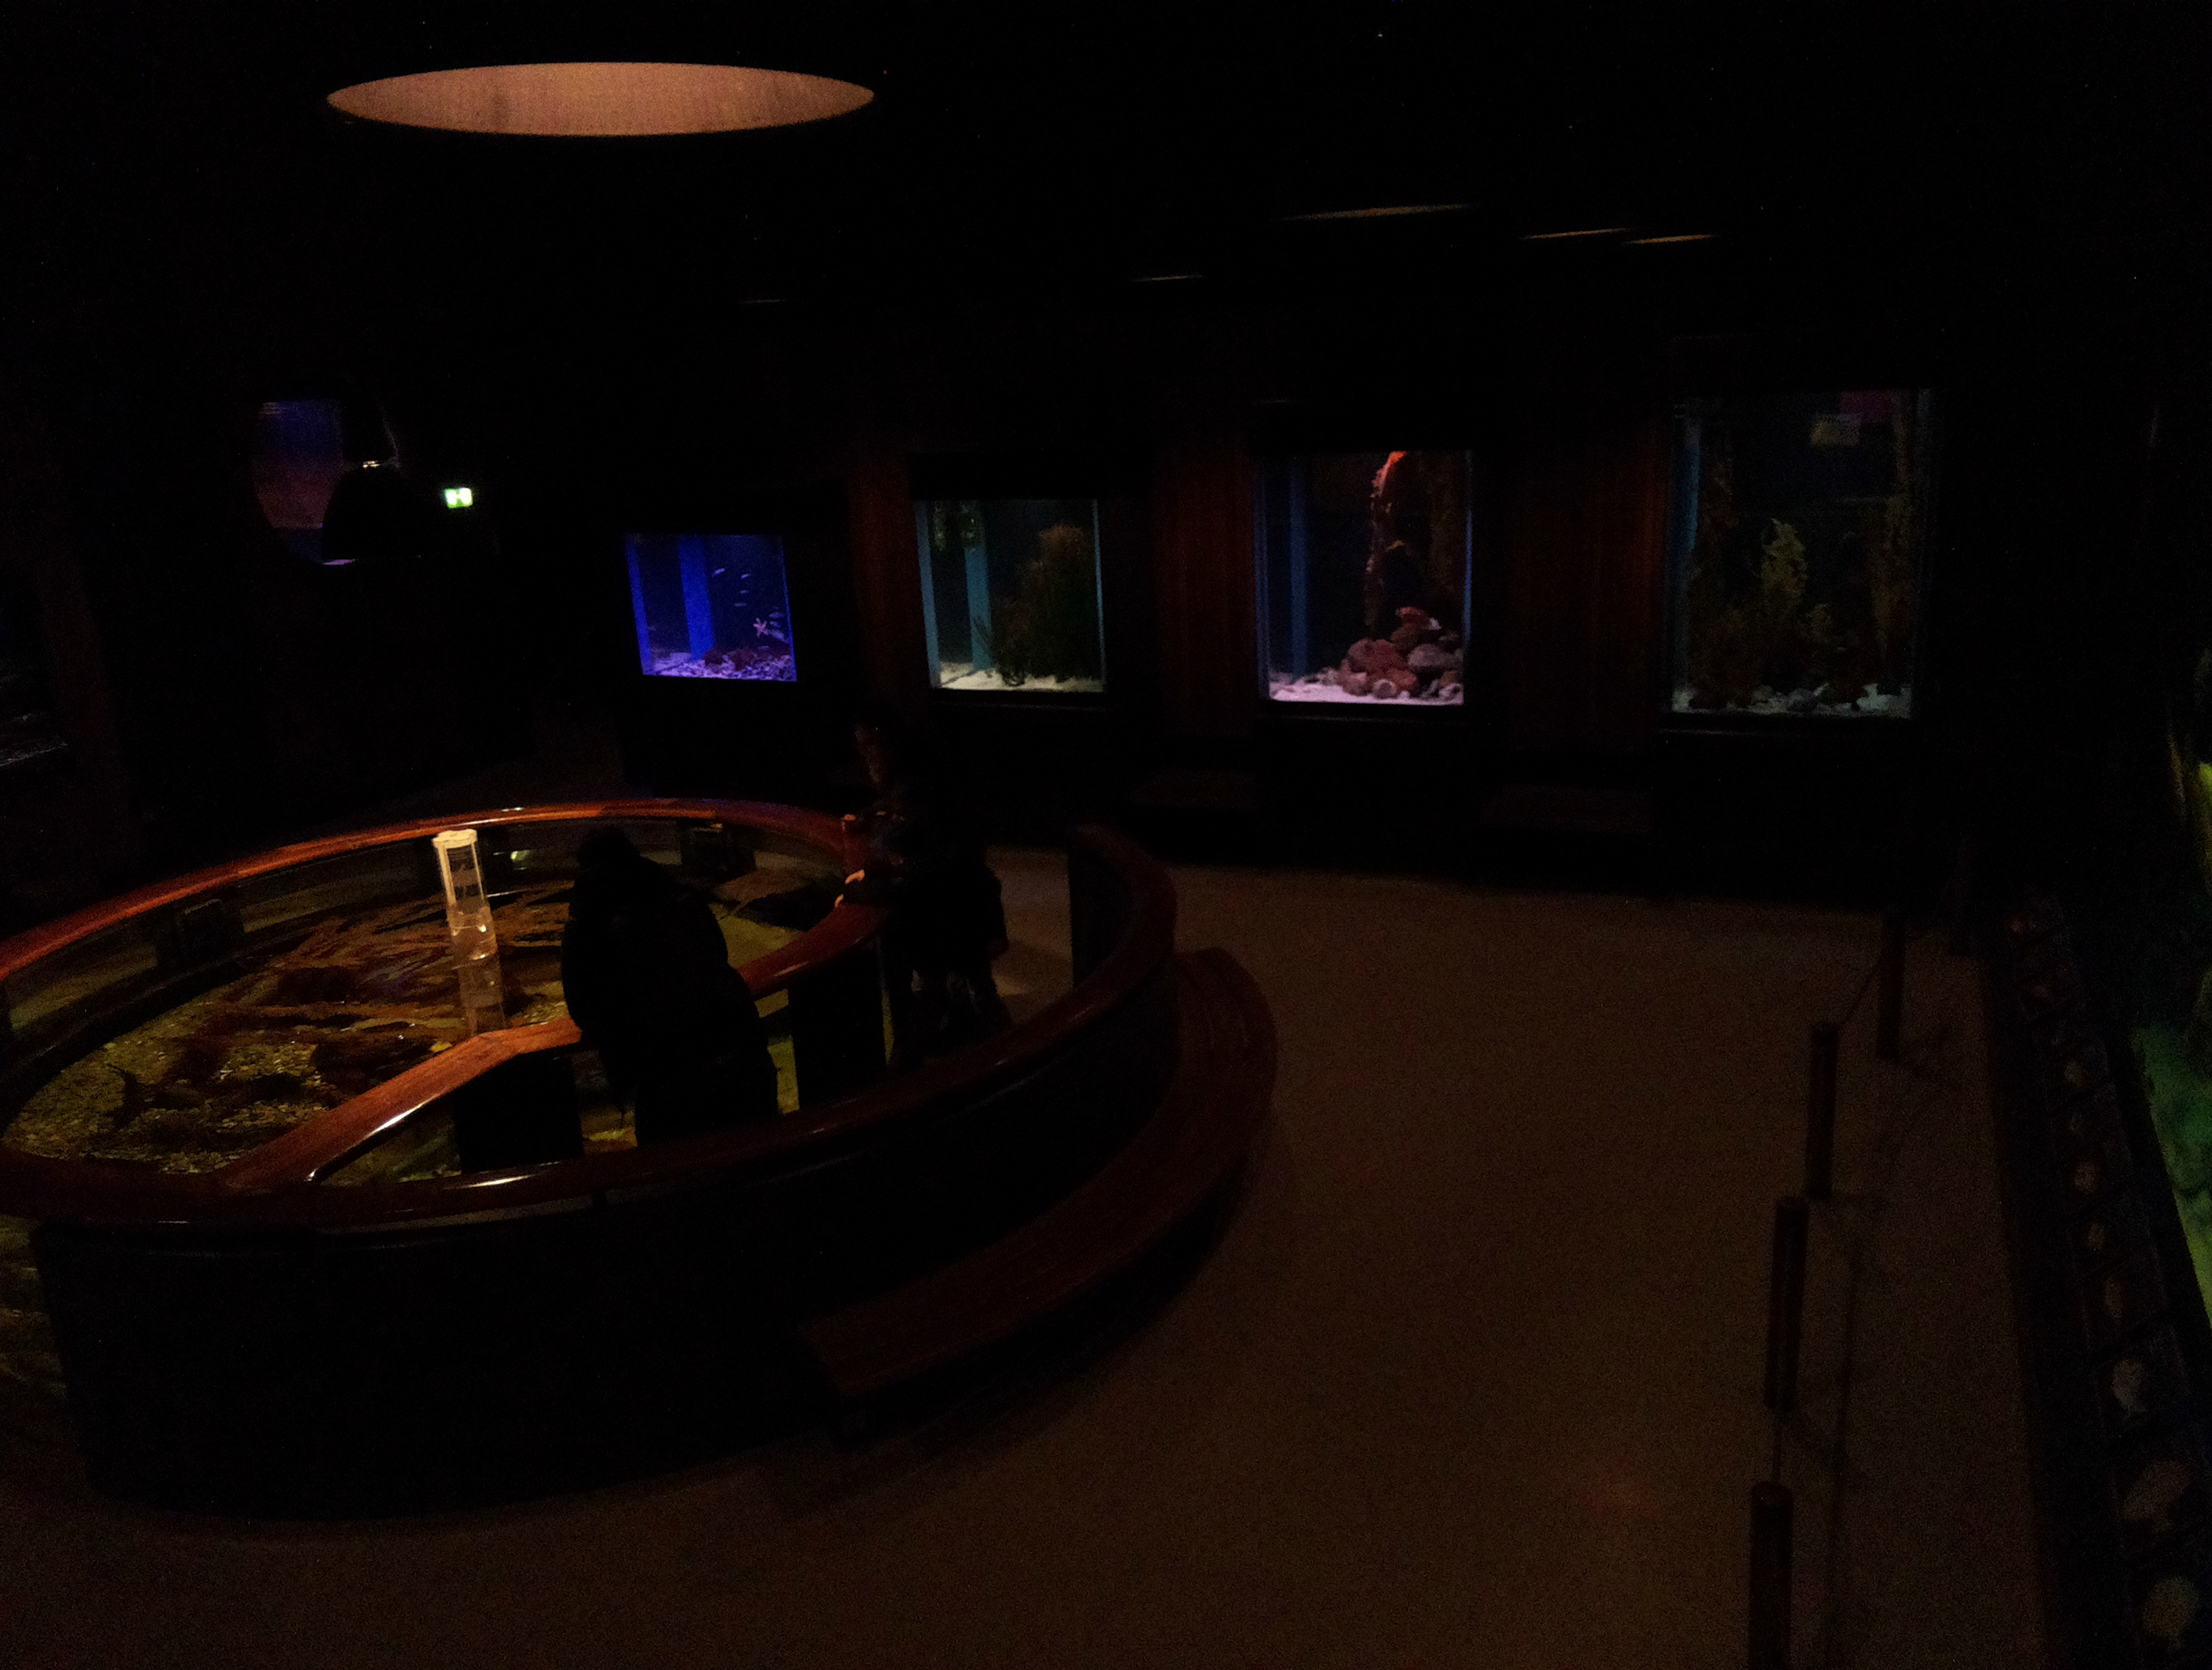
\includegraphics[options]{Images/DeviceImages/2nd-iteration/ss20000_fimus.jpg}

% \end{figure}

\textbf{3rd iteration}
\textit{Total number of images: TODO. 1 subject.}
For the third iteration the camera setup was better prepared. Two main differences since the last iteration was made. The first was to opt for a higher post-processing brightness value and a faster exposure speed to increase the number of images taken. The other was to spend some time beforehand setting up the camera to the best position before starting image capture. The image capture sessions are heavily influenced by the constraint of not photographing unconsenting individuals, thus limiting the capturing session to the windows where no other persons are in the acquarium. Therefore, spending time setting up the camera and verifying it's positioning is time which could be spent capturing images for the dataset. However, with well-enough time to complete the project, spending some extra time setting everything up correctly can save time in later stages of the process. 

The third iteration was made after setting everything up, in the time waiting for a second subject arrive.

\textbf{4th iteration}

The 4th iteration was with the same exact setup as the 3rd iteration, but with 2 subjects instead of 1.  

\subsection{Labeling}
\label{sec:labeling}
The detector needs to know the ground truth of the correct person positions when training and validating on the images. 

The images was first inferenced by a yolov9 detector pre-trained on the COCO dataset. This is a way to greatly speed up the labeling process, instead of manually labeling every image. The detector had close to zero hallucinations due to a sufficiently high confidence rate of 0.5. Out of the 2939 images in the 1st-iteration dataset, 1076 came out with no detections and had to be manually labeled. The rest of the images were then validated. In 74 of the images, a part of one the fish tanks were identified to be human, as it was a moving seaweed that sometimes had a human-like shape. In one image the person was carrying a ladder which was identified to be a person. 

The 2nd iteration images were brighter, and in these images one of the roof-lamps were sometimes identified to be human.

In one image, the lamp and the seaweed were the only persons in the image. insert 120324-163917-84. 
In another, the seaweed was more man than I. 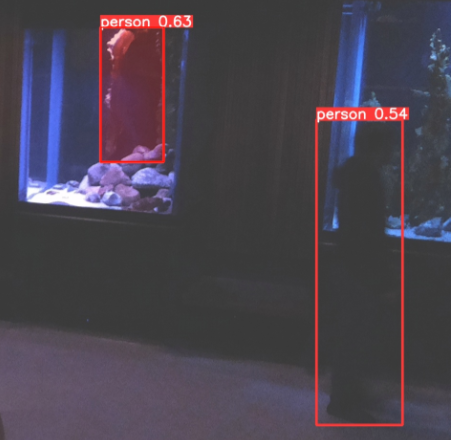
\includegraphics[width=0.4\textwidth]{Images/fun/seaweed-man-more-than-I.png}.

TODO hører hjemme i en recommendations eller discussion? selv-kritiske kommentarer.. I forstudien hadde jeg en "reflections" etter diskusjon som sa litt om hva jeg ville gjort anerledes og forklarte noen av de valgene jeg tok. 
The time to understand the tools and develop this pipeline was similar to what it would take to manually label all the images, but can now be used for future applications also. The approach to label the images is described in section: \ref{sec:labeling}.

After the ground truth was identified for all the dataset images, it was then used to evaluate the pre-trained yolov3 and yolov9. Results are discussed in \ref{sec:results}. The data was then used to train the detectors. The training process is described in section \ref{sec:model_training}. The trained models were then deployed to the device to evaluate the inference speed and accuracy.

To visualize the improvements and highlight the areas in the image benefitting most from detector improvements, heat maps were generated. The process of generating heat maps is described in section \ref{sec:heatmaps}.


"Label Studio" was used to label the images. 

Labeling speed: about 10 images per minute, when calculating in the time of deleting images without people,

\subsection{Model Training}
\label{sec:model_training}

\subsubsection{Hyperparameter Optimization}
todo finskriv... Not really optimization.. More like finding... Since we're doing a cheeky approach to this. Done with autogluon, follow this guide for installation: https://auto.gluon.ai/stable/install.html. I had to run pip install autogluon twice for the imports to see autogluon.

This guide could be used to fine tune the hyperparameters of the model: https://auto.gluon.ai/scoredebugweight/tutorials/course/script.html. A simpler guide was implemented to find the hyperparameters. This was to save time, and since our models require an okay level of hyperparameters. However, this choice to not give every dataset the same "fighting chance" with their optimal hyperparameters might have led to a lower validity of this experiments results. 

The hyperparameters were optimized for a yolov3 fitting to the 2nd iteration dataset, which was used for evaluation of all the models. To do this, the 1st iteration dataset was used for training data and the 2nd iteration dataset was used for validation data. No data was saved for testing, as this model was trained only to find the best hyperparameters.


\subsection{Ethical Considerations}
In the deployment of advanced machine learning technologies for visitor localization and engagement analysis, this research proactively addresses privacy concerns through the implementation of image obscuration techniques. These methods ensure that no personally identifiable information is captured or communicated, thus significantly reducing privacy risks associated with visitor tracking in cultural spaces such as museums and aquariums.

\subsubsection{Privacy by Design}
At the forefront of our ethical approach is the principle of "privacy by design." This concept involves integrating privacy into the development and operation of our tracking technologies from the outset, rather than as an afterthought. By employing image obscuration techniques, such as real-time pixelation or silhouette generation, we ensure that the visual data processed by our system remains anonymous. This method effectively eliminates the possibility of identifying individual visitors from the captured data, thereby safeguarding their privacy.

The application of these privacy-preserving techniques negates the need for explicit consent from visitors for two primary reasons. First, the anonymization process occurs instantaneously as the data is captured, meaning no identifiable information is ever stored or analyzed. Second, the focus of the research is on aggregate behavior patterns rather than individual actions, further distancing the study from privacy concerns.

\subsubsection{Ethical Use and Data Protection}
Ensuring the ethical use of technology extends beyond privacy considerations to include the responsible handling and protection of any data generated by the system. Although the data is anonymized, we are committed to maintaining high standards of data protection. This includes secure data storage, limiting access to authorized personnel, and employing robust data management policies that comply with relevant data protection laws and guidelines. 

The utilization of anonymization techniques also reflects our commitment to minimizing any potential impact on visitor behavior and the overall museum or aquarium experience. By ensuring that the tracking system is unobtrusive and does not compromise privacy, we aim to maintain the integrity of the visitor experience, allowing individuals to engage with exhibits without concern for their privacy.

\subsubsection{Transparency and Accountability}
While the technical approach effectively addresses privacy concerns, maintaining transparency about the use and purpose of tracking technologies is still essential. Information about the tracking system and its privacy-preserving nature will be made available to visitors, ensuring they are informed about how data is used to enhance the visitor experience.

Furthermore, the project will adhere to an ongoing ethical review process, ensuring that all aspects of the research remain aligned with ethical best practices and respond to evolving technological and societal standards.

In summary, by prioritizing privacy through the use of image obscuration techniques and adopting a comprehensive ethical framework, this research aims to advance the understanding of visitor engagement in a manner that is both innovative and respectful of individual privacy rights. This approach sets a precedent for the ethical application of machine learning technologies in cultural institutions, balancing the benefits of visitor behavior analysis with the imperative of protecting privacy.


\subsection{Heatmaps}
\label{sec:heatmaps}

\subsection*{Notes}
Tried to download/use model from Roboflow, but either image has to be sent to an API which would not retain privacy, or the device has to host an API itself to run the inference... Seems unlikely to be the most preferable solution, as the device would have to set up the service and run it locally. Possibly an interesting solution would be to do this with multiple devices. This supports the master-slave pattern of having multiple weaker computers and have them send to the stronger unit. Setting up private TCP connection between the weaker units and the strong unit and have the images sent to the stronger, so it can detect on them and send information etc... How many weak units do we need in order to make it profitable to have a strong GPU unit to do the processing? This whole systems sounds to be complicating processes, not making the product modular and easy-to-use. Includes a lot of connection/networking to make the weaker units find and connect to strong, physically close device.
    This task would mean setting up a strong device to host a network to which the weak units might connect to, and send images to. The issue is whenever images are sent, a lot of transmission is used... But the model takes image input size of 416x416. Would it be similar to just downscale the image before sending, or would this give the model less detail to work with?

Will now run several models on datasets from the web, i.e. the CrowdHuman dataset to see their accuracies. Will then deploy the models to device in acquarium to see if the best-performing model is an option in terms of size and inference speed. If it is preferable, I will attempt to increase it's accuracy by accumulating and annotating a specialized dataset for that setting, and training the final layers on the data. Can this be done with a 